% Chapter Template

\chapter{Reti Neurali Convoluzionali} % Main chapter title

\label{Capitolo2} % Change X to a consecutive number; for referencing this chapter elsewhere, use \ref{ChapterX}
%variables to define path to images
\def \teoria {Figures/teoria}

%--------------------------------------------------------------------%	SECTION 1
%--------------------------------------------------------------------

\section{Breve introduzione}
La reti neurali convoluzionali, alle quali ci riferiremo con l'abbrevazione \emph{CNN} - dall'inglese \emph{Convolutional Neural Network}, sono un'evoluzione delle normali reti artificiali caratterizzati da una particolare architettura che le ha rese negli anni molto efficaci su diversi compiti. 


\begin{figure}[h!]
 \centering
 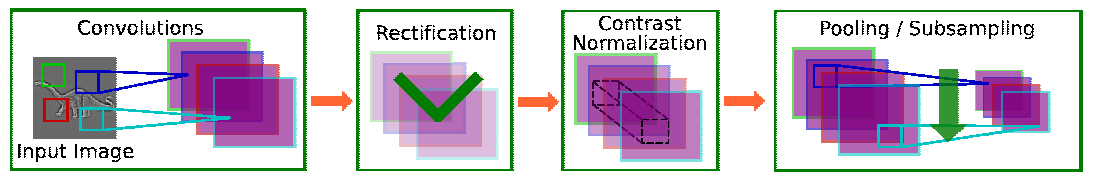
\includegraphics[width=1.0\textwidth]{\teoria/CNN-features.png} 
 \caption{I diversi strati tipici di una CNN}
 \label{fig:conv1}
\end{figure}

%--------------------------------------------------------------------
%	SECTION 2
%--------------------------------------------------------------------

\section{Architettura}
\subsection{Strato di Convoluzione}

\subsection{Strato di Pooling}

\subsection{Strato completamente connesso (FC)}


%--------------------------------------------------------------------
%	SECTION 3
%--------------------------------------------------------------------

\section{Applicazioni e risultati}


